\chapter{Feature Design} \label{sec:feature}

	% Chapter overview of sections
	% Chapter overview of sections
	% Chapter overview of sections

	% Introduction into sections
	\section{System Overview}

		\paragraph{What is OASIS}
			% What is OASIS
			% What is your objective with oasis
			The online architectural sketching interface for simulations (OASIS) is intended to be a  general early design tool for both novices and architects. OASIS provides a platform independent sketching interface that generates closed 3D triangle meshes with optimal properties for simulations. Currently, OASIS only supports daylighting visualizations; however, OASIS can be extended to support other simulations that make use of closed triangle meshes, including acoustic and thermal simulations. The main advantage OASIS offers users is an novel interface that does not require detailed geometric modeling for the creation of 3D triangle mesh models and an interface to analyze simulation results. An additional advantage of using OASIS is the client-server architecture that allows users to be able to run computationally expensive simulations at interactive rates regardless of their machine specifications.

		\paragraph{Virtual Heliodon Pipeline}
			% <Pipeline of the Virtual Heliodon>
			Both OASIS and the Virtual Heliodon provide a novel solution to the challenge of daylighting analysis during the early stage of architectural design.
			In addition to sharing the same objectives both OASIS and the Virtual Heliodon utilize the physical sketch interpretation algorithm and the daylight rendering engine.
			As a result it can be difficult to see where these two systems vary.
			In order to understand the contributions I made to OASIS we must briefly cover the system pipeline of the Virtual Heliodon.
			The Virtual Heliodon's system pipeline is illustrated in Figure-\ref{pipeline_vh}.
			To begin, the Virtual Heliodon features a novel tangible user interface for the creation of architectural spaces.
			Users define architectural spaces by manipulating physical foam primitives with their hands.
			After users are satisfied with their architectural space they can either use a wireless clicker or communicate to the operator to run the \textit{table top detect} process and continue to generate a closed triangle mesh from their physical sketches; Communication with the operator to run the \textit{table top detect} process is noted in Figure-\ref{pipeline_vh}A.
			The \textit{table top detect} processes is a simple computer vision program that takes an overhead image of the foam primitives and detects where those primitives are in an image.
			The coordinates of where those primitives are in an image are stored in an intermediate primitives file. The intermediate primitives file is used as input for the physical sketch interpretation algorithm. As mentioned previously, the physical sketch interpretation algorithm generates a closed watertight triangle mesh.
			Currently, there exist no user interface for the generation of daylight visualizations.
			Instead, an operator familiar with the system is required to generate visualizations for users, as shown in Figure-\ref{pipeline_vh}B.
			After the generation of watertight 3D models, users communicate to the operator the time and date they would like visualized. 
			Depending on the time,date, and user visualization requested the operator would manually modify existing scripts to generate those visualizations on the Virtual Heliodon.
			These scripts would include invoking the daylight rendering engine to generate image textures to be projected onto users' physical sketches.
			In other words, the Virtual Heliodon does not offer much autonomy and requires an operator to both explain how to use the tangible user interface and constantly communicate with users to operate the Virtual Heliodon.
			% </Pipeline of the Virtual Heliodon>

  		\begin{figure}[h]
			\centering
			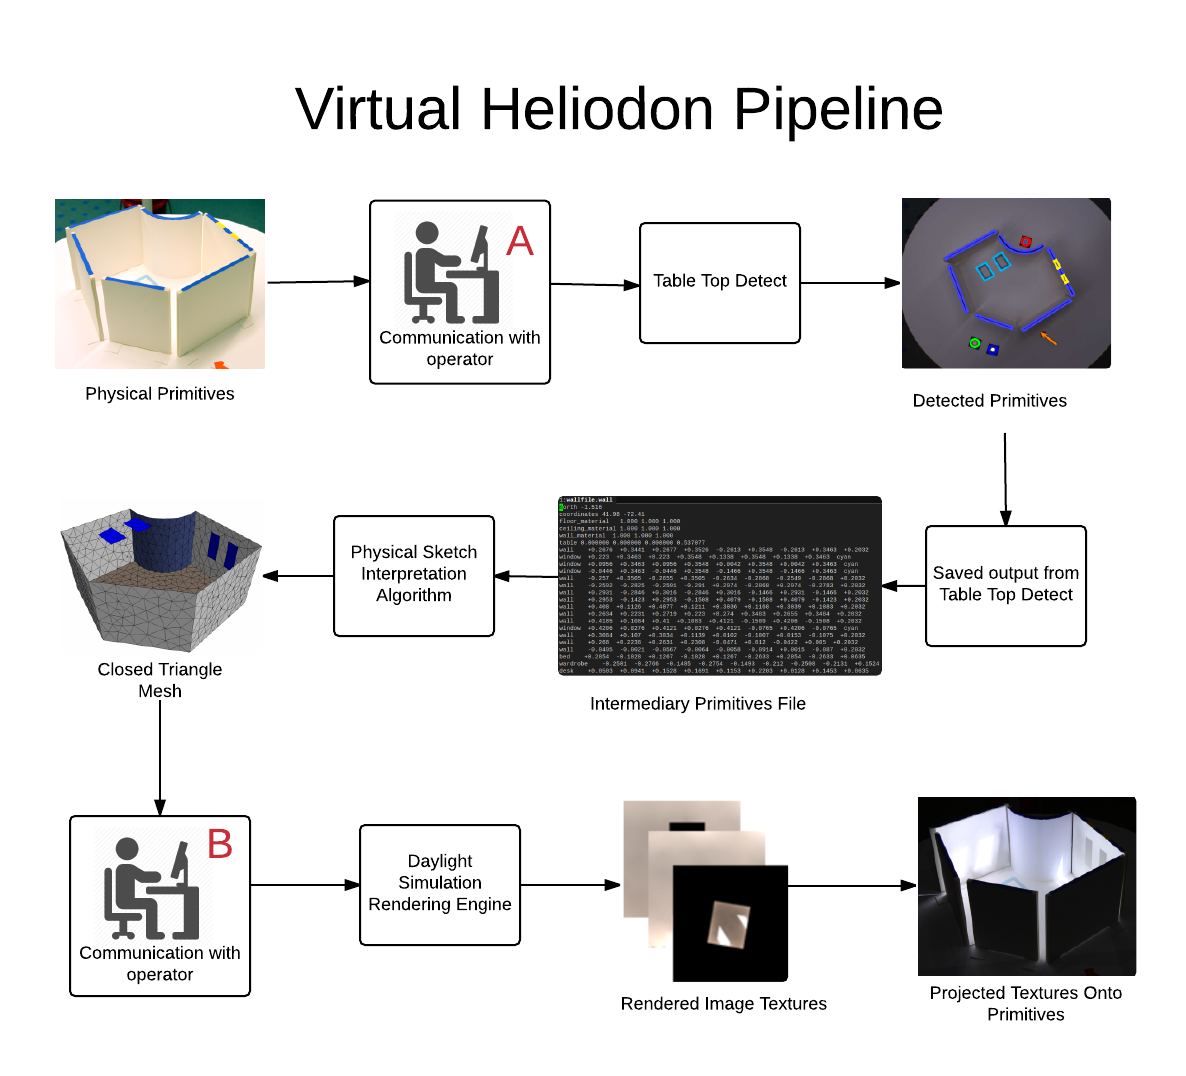
\includegraphics[width=1.0\textwidth]{pipeline_vh}
			\caption{Virtual Heliodon's simplified pipeline. A and B are locations in the pipeline that require an experienced operator to perform technical actives on the Virtual Heliodon. }
			\label{fig:new_pipeline}
			\end{figure}

		\paragraph{OASIS Pipeline}
			OASIS is an alternative interface to the Virtual Heliodon. 
			The system pipeline in Figure-\ref{fig:new_pipeline} illustrates the components involved in OASIS.
			In addition, Figure-\ref{fig:new_pipeline} emphasizes all portions of OASIS that I directly contributed to.
			To begin, users on OASIS generate 2D sketches consisting of lines that represent wall and windows and objects that represent furniture items.
			The physical sketch interpretation algorithm that the Virtual Heliodon uses to generate watertight 3D meshes for simulations require sketches be given as a collection of model primitives. 
			Therefore, before being able to invoke the physical sketch interpretation algorithm, OASIS generates the intermediate primitives file.
			Model primitives are stored in an intermediate primitives file where each line describes a wall,window, or furniture item in a sketch.
			As mentioned previously, in the Virtual Heliodon the intermediate primitives file is created by a simple computer vision algorithm that detects walls, windows, and tokens through colored markers placed on the top of physical primitives.
			Since the sketching interface is purely in-software, I can directly create this intermediate primitives file without need of a computer vision algorithm to detect primitives.
			Interestingly, OASIS avoids a few limitations on the Virtual Heliodon by bypassing the need to detect physical primitives. 
			OASIS can support a wider vocabulary of primitives because it is not bound to the detection of color tokens.
			Additionally, at certain angles parallel wall primitives in close proximity to each other on the Virtual Heliodon could result in the occlusion of primitives in the overhead image. 
			Since OASIS is an in-software solution this problem is avoided as the position of all primitives is always known.
			Figure-\ref{fig:new_pipeline}A illustrates where OASIS generates the intermediate primitives file in our system pipeline.
			Given the intermediate primitives file the physical sketch interpretation algorithm outputs a closed triangle mesh that the user can view in the \textit{Generate 3D Model} page.
			Given the user's confirmation that a 3D generated model matches user's intention, the user can create a daylight simulation request in the \textit{Create Daylighting Simulation} page.
			This portion of the system pipeline is illustrated in Figure-\ref{fig:new_pipeline}B.
			After the submission of a daylight simulation request, I use the daylight simulation rendering engine to produce texture images.
			These texture images capture global illumination from a daylight simulation in a viewpoint independent manner.
			On the \textit{Analyze Daylighting} page, I map these texture images onto the 3D mesh to display a daylight rendering of the user's generated model.
			Figure-\ref{fig:new_pipeline}C illustrates where texture mapping occurs in the system pipeline.
			In brief, our pipeline shows that OASIS is an alternative autonomous interface to the physical sketch interpretation algorithm and daylight rendering engine in the Virtual Heliodon.

			\begin{figure}[h]
			\centering
			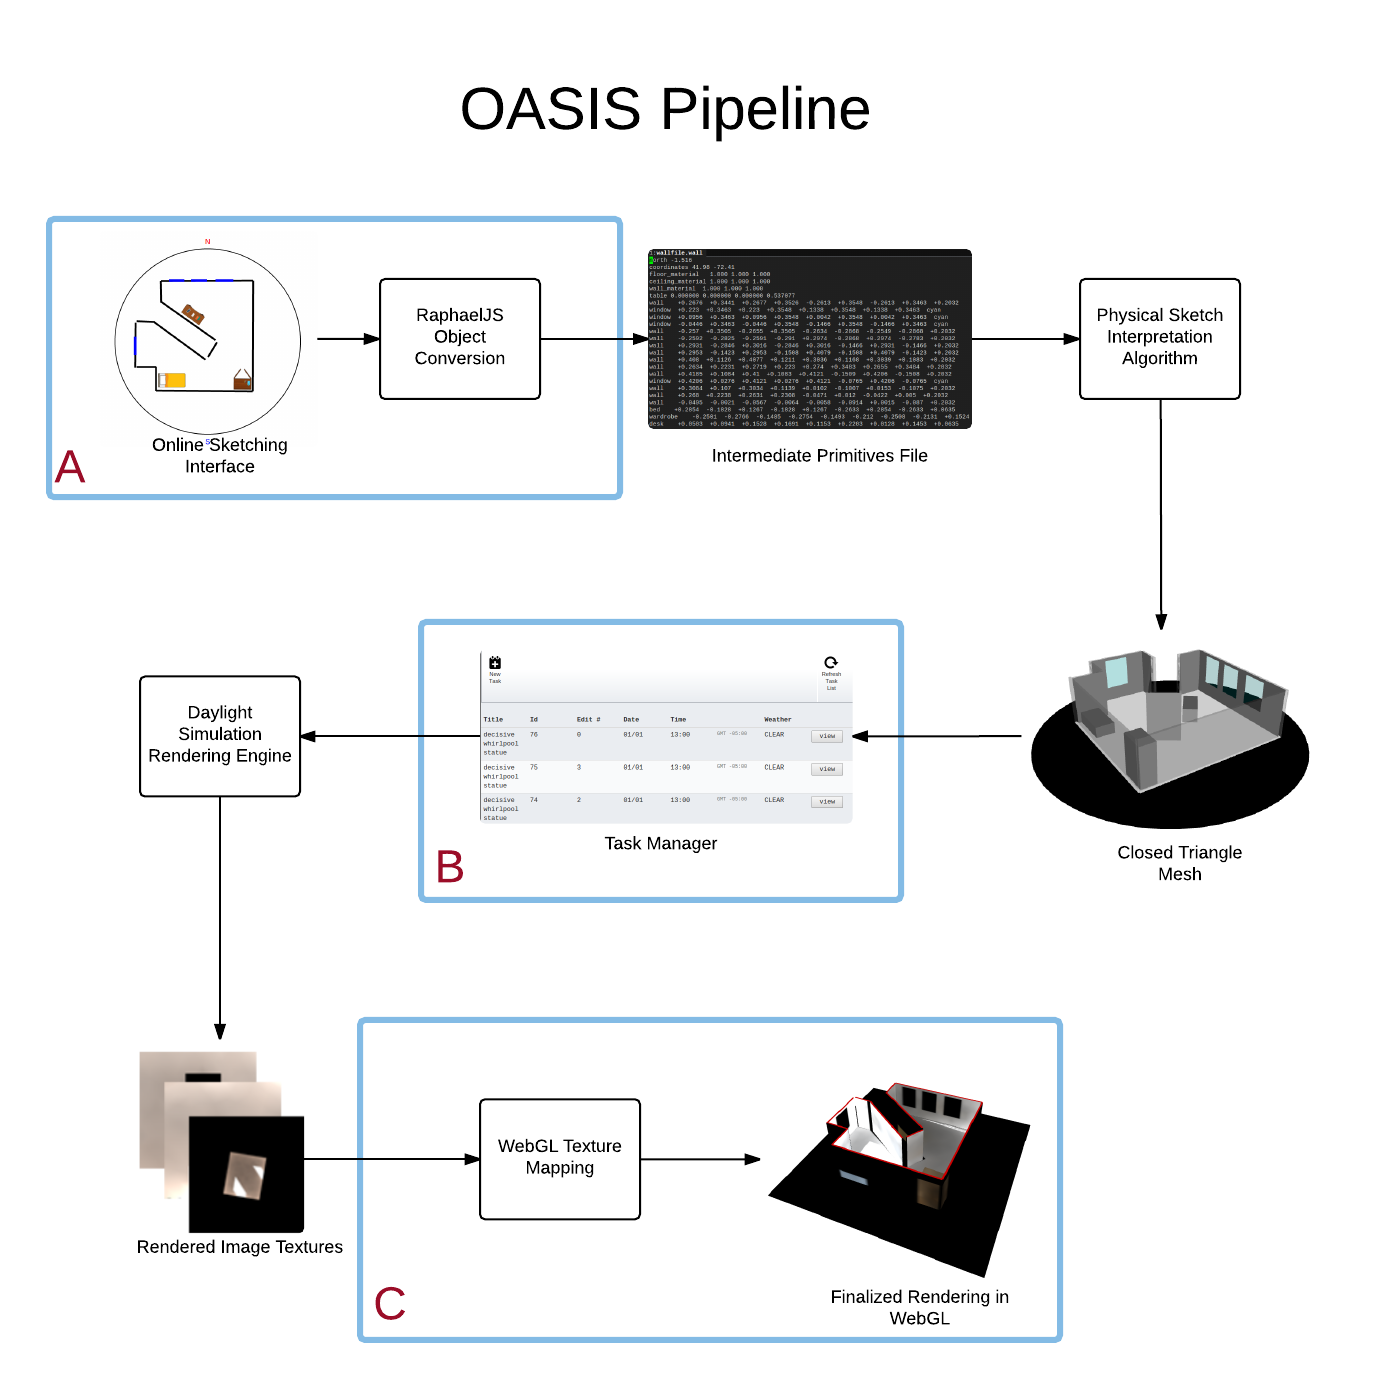
\includegraphics[width=1.0\textwidth]{new_pipeline}
			\caption{OASIS pipeline diagram with the author's contributions noted in blue.}
			\label{fig:new_pipeline}
			\end{figure}

		\paragraph{Importance of UI}
		OASIS is intended to provide an easy-to-use  and autonomous interface for interacting with the physical sketch interpretation algorithm and daylight rendering engine. 
		As discussed previously, the interface in the Virtual Heliodon requires an experienced operator at all times.
		It is important to note that there has been attempts to give users control over the Virtual Heliodon including programming a remote clicker to trigger the \textit{table top detection} process.
		However, there is currently no user interface for choosing visualizations to display and define the parameters required by those visualizations.
		The Virtual Heliodon, just like OASIS, aims to be an easy-to-use interface for not only the design of architectural spaces but also the generation of helpful visualizations.
		Requiring an operator with programming experience and background knowledge on Virtual Heliodon may hinder the usage of the tool.





	\section{Sketching Interface Design}
		\paragraph{Sketching Walls and Windows}
			% Why is sketching walls/win important
			% Discussion about what we do
			% Discussion about alternatives(old method)
			% Discussion about Eric's work
		\paragraph{Furniture Placement}
			% Why is furniture important
				% Scale
				% Meaning (identity)
				% Relate to space
			% Discussion about how we place furniture
			% Discussion about furture work on sketched furniture items
				% Dynamic scale??
		\paragraph{Removal of Elements}
			% Why is removal important
				% side: machines do better removal than pen & paper
			% How do we implement it
			% Alternatives
		\paragraph{Cardinal Orientation}
			% Why is orientation important
			% How do we implement it? 
			% Alternatives
		\paragraph{Geographical Positioning}
			% Why is location important
			% How do we implement it? 
			% Alternatives

	\section{3D model viewer}

		\subsection{Physical Sketch Interpretation Algorithm Viewer}
			\paragraph{Intention}
			\paragraph{Examples of successful interpretations}
			\paragraph{Examples of unsuccessful interpretations}

		\subsection{Daylight Rendering engine viewer}
			\paragraph{Examples of successful interpretations}
			\paragraph{Examples of unsuccessful interpretations}
				\paragraph{Examples of over illuminatioh}
				\paragraph{Examples of under illuminatioh}

		\subsection{Share a Model viewer}
			\paragraph{Purpose of Model Viewer}
			\paragraph{Alternatives?}

	\section{Web Application Design}
		\paragraph{Why is good UI important for our application}
		\paragraph{General User Interface choices}
		\paragraph{Non-Linearity in OASIS}
		\paragraph{Loading Previous Models and Rendering Task}

	\section{Problems Encountered}
		\paragraph{Computational Intensive Procedures}
		\paragraph{Saving Models Safety}
		\paragraph{Dealing with Clueless Users}

	\section{Implementation}

		\subsection{Frameworks Used}
			\paragraph{WebGL}
			\paragraph{RaphaelJS}
				Another framework used in our sketching interface is RaphaelJS\cite{todo}.
				Raphael JS is a 3D vector graphics library for JavaScript. 
				I use RaphaelJS to create 2D graphics of objects users places into sketches. I also use RaphaelJS because it supports vectorized lines and shapes, allowing our interface  to be re-sizable with lost of visual quality.
				I also use Raphael FreeTransform in conjunction with RaphaelJS\cite{todo}. 
				The FreeTransform extension is used to create FreeTransform handles on furniture items so that users may easily rotate and reposition furniture items where they please.
				Figure-\ref{fig:oldvh}F demonstrates the handles FreeTransform generates for object manipulation.\\


			\paragraph{RibbonJS}


		\subsection{Window Snapping}

	\section{Chapter Summary}
		% Summary of what we covered

